\chapter{Latency Reduction\label{chap4}}

Previous chapter demonstrated virtual interrupt latency for real-time guest is significantly larger than in native setup.
Recent extensions to x86 hardware-assisted virtualization support virtualization of local interrupt controller (APIC-v) 
that enables hypervisor to minimize its involvement. Furthermore, it allows direct interrupt injection to the guest for
devices that are owned by guests. It also enables virtualization of translation lookaside buffers (TLBs) by supporting virtual
process identifiers (VPIDs). Hypervisor can use VPIDs to isolate address translation information of different guests from each other and from hypervisor.
Intel Cache Allocation Technology addresses contention of shared LLC that enables hypervisor to partition shared cache
between the guests to avoid cache pollution.
This chapter presents results of using these hardware mechanisms to reduce interrupt latencies for real-time guest.
Following sections provide details of using each mechanism separately and records improvements in the interrupt latency.


\section{Direct Interrupt Injection}
Direct interrupt injection (DII) mechanism allows guest operating system to receive interrupts from 
external devices without hypervisor involvement.
APIC virtualization allows hypervisor to deliver virtual interrupts directly to the guest code without causing a trap. 
The details of this feature has already been covered in section \ref{sec:dii}.
A brief summary of the mechanism is as follows.
Hypervisor can marks a virtual interrupt as a posted interrupt (PI) in posted interrupt-descriptor (PID). 
PID is a data structure allocated by hypervisor.
It allows hypervisor inform interrupt controller that an interrupt is owned by guest and has to be delivered to guest without hypervisor involvement. 
Posted interrupt mechanism only works when hypervisor uses APIC virtualization to manage guest interrupts. 
Figure \ref{fig-posted-interrupts} demonstrates delivery of a guest interrupt does not require hypervisor involvement if it is marked as PI.
Succeeding sections describe performance evaluation of the real-time guest interrupt when DII is used.

\begin{figure}[!htb]
\begin{center}
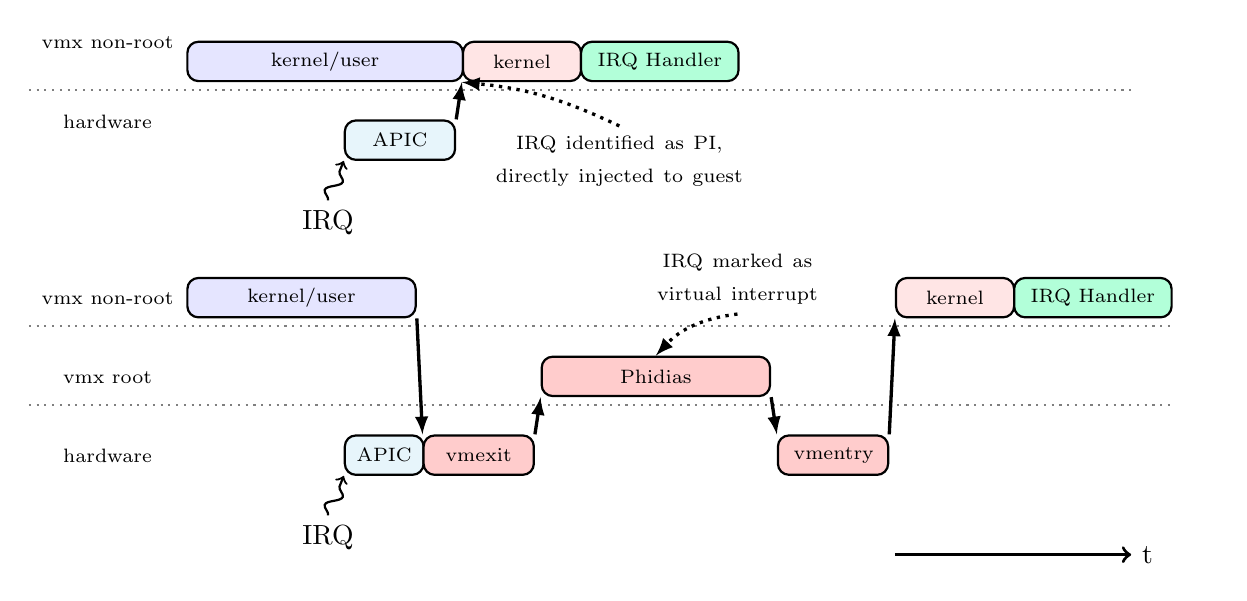
\begin{tikzpicture}

%\draw[step=1cm, gray, very thin, dotted] (-1,-1) grid (10,6);

\draw[black, very thick, ->] (9,-1) -- (12,-1) node [below, right] {t};
\draw[black, thick, dotted, opacity=0.5] (-2,0.9) -- (12.5,0.9) node at (13,0.9) [below] {};
\draw[black, thick, dotted, opacity=0.5] (-2,1.9) -- (12.5,1.9) node at (13,1.9) [below] {};
\node at (-1, 2.25) {\scriptsize{vmx non-root}};
\node at (-1, 1.25) {\scriptsize{vmx root}};
\node at (-1, 0.25) {\scriptsize{hardware}};


\node at (0,2) [rectangle, draw=black, thick, fill=Blue!10, rounded corners, minimum height = 0.5cm, minimum width = 2.9cm, anchor=south west] (kubefore) {\scriptsize{kernel/user}};
%\draw[black, thick, dashed, opacity=0.7] (1.95,-0.25) -- (1.95, 3.0)  node [above, text width = 1cm] {IRQ};
\node at (2,0) [rectangle, draw=black, thick, fill=SkyBlue!20, rounded corners, minimum height = 0.5cm, minimum width = 1cm, anchor=south west] (apic) {\scriptsize{APIC}};
%\draw[black, thick, dashed] (3.0,-0.25) -- (3.0, 3.75)  node [above, text width = 4cm] {IRQ not marked as PI};
\node at (3,0) [rectangle, draw=black, thick, fill=Red!20, rounded corners, minimum height = 0.5cm, minimum width = 1.4cm, anchor=south west] (vmexit) {\scriptsize{vmexit}};
\node at (4.5,1) [rectangle, draw=black, thick, fill=Red!20, rounded corners, minimum height = 0.5cm, minimum width = 2.9cm, anchor=south west] (phidias) {\scriptsize{Phidias}};
\node at (7.5,0) [rectangle, draw=black, thick, fill=Red!20, rounded corners, minimum height = 0.5cm, minimum width = 1.4cm, anchor=south west, text width=1cm] (vmentry) {\scriptsize{vmentry}};
%\draw[black, thick, dashed] (7.5,-0.25) -- (7.5, 3.25)  node [above, text width = 4cm] {IRQ marked pending};
\node at (9,2) [rectangle, draw=black, thick, fill=red!10, rounded corners, minimum height = 0.5cm, minimum width = 1.5cm, anchor=south west] (kafter) {\scriptsize{kernel}};
\node at (10.5,2) [rectangle, draw=black, thick, fill=SpringGreen!30, rounded corners, minimum height = 0.5cm, minimum width = 2cm, anchor=south west] (irqhandler) {\scriptsize{IRQ Handler}};
\draw[thick, decorate, decoration=snake, ->] (1.8, -0.5) -- (2, 0) node at (1.8, -0.5) [below] {IRQ};


\node at (7,2.5) (irqvi) [text width=4cm, align=center] {\scriptsize{IRQ marked as virtual interrupt}};
\node at (5.5,4) (irqpi) [text width=4cm, align=center] {\scriptsize{IRQ identified as PI, directly injected to guest}};

\begin{scope}[>=latex]
	%\draw [thick, ->] (kubefore.south east) to [bend right=0] (vmexit.north west);
	\draw [very thick, ->] (kubefore.south east) -- (vmexit.north west);
	\draw [very thick, ->] (vmexit.north east) -- (phidias.south west);
	\draw [very thick, ->] (phidias.south east) -- (vmentry.north west);
	\draw [very thick, ->] (vmentry.north east) -- (kafter.south west);
	\draw [very thick, dotted, ->] (irqvi.south) to [bend right=20] (phidias.north);
	
\end{scope}

\draw[black, thick, dotted, opacity=0.5] (-2,8-3.1) -- (12,8-3.1) node at (13,8-3.1) [below] {};
\node at (-1, 8-2.5) {\scriptsize{vmx non-root}};
\node at (-1, 8-3.5) {\scriptsize{hardware}};

\node at (0,8-3) [rectangle, draw=black, thick, fill=Blue!10, rounded corners, minimum height = 0.5cm, minimum width = 3.5cm, anchor=south west] (kubefore2) {\scriptsize{kernel/user}};
%\draw[black, thick, dashed, opacity=0.7] (1.95,-4.25) -- (1.95, -2.0)  node [above, text width = 1cm] {IRQ};
\draw[thick, decorate, decoration=snake, ->] (1.8, 8-4.5) -- (2, 8-4) node at (1.8, 8-4.5) [below] {IRQ};
\node at (2.0,8-4) [rectangle, draw=black, thick, fill=SkyBlue!20, rounded corners, minimum height = 0.5cm, minimum width = 1.4cm, anchor=south west] (apic2) {\scriptsize{APIC}};
%\draw[black, thick, dashed] (3.5,-4.25) -- (3.5, -1.5)  node [above, text width = 4cm] {IRQ recognized as PI};

\node at (3.5,8-3) [rectangle, draw=black, thick, fill=red!10, rounded corners, minimum height = 0.5cm, minimum width = 1.5cm, anchor=south west] (kafter2) {\scriptsize{kernel}};
\node at (5.0,8-3) [rectangle, draw=black, thick, fill=SpringGreen!30, rounded corners, minimum height = 0.5cm, minimum width = 2cm, anchor=south west] (irqhandler2) {\scriptsize{IRQ Handler}};

\begin{scope}[>=latex]
	\draw [very thick, ->] (apic2.north east) -- (kafter2.south west);
	\draw [very thick, dotted, ->] (irqpi.north) to [bend right=10] (kafter2.south west);
\end{scope}


\end{tikzpicture}
\end{center}
\ifreport
\caption{Posted interrupt versus virtual interrupt delivery}
\fi
\label{fig-posted-interrupts}
\end{figure}



\subsection{Methodology}
Performance evaluation setup for direct interrupt injection mechanism includes PREEMPT\_RT patched Linux as real-time guest (rt-guest)
and Linux as general-purpose guest (gp-guest). Each guest is assigned to a separate core and has access to 256MB of RAM. The setup is 
similar to the one described in section \ref{sec:methodology}, rt-guest has direct access to PCIe gpio card capable to generate interrupts. 
Measurement setup is same as described in section \ref{sec:measurement-setup}.
Phidias hypervisor was extended to use direct interrupt mechanism for rt-guest GPIO interrupt.
PID data structure has an outstanding notification (ON) bit that enables DII logic. 
The ON bit is cleared by hardware after injecting a posted interrupt directly to the guest. 
The hypervisor is responsible to set the bit again before arrival of posted interrupt, if it fails the interrupt is delivered to hypervisor.
Since external gpio interrupts events are generated at rate of about 1ms, hypervisor was informed by causing an intentional exit from interrupt handler to
set ON bit again. The approach is similar to the one used in section \ref{sec:context-switch-overhead}.
The latency reduction is evaluated by measuring worst-case interrupt latency with and without direct interrupt mechainsm.
It involves generating ten thousand GPIO interrupts and recording latency of each event.

\subsection{Latency Reduction}
\begin{figure}[!htb]
\begin{center}
\begin{tikzpicture} [
						my brace/.style={thick, decorate, decoration={brace, amplitude=4pt, raise=10pt,},},							
						my label/.style={below right, align=center, rotate=90, inner ysep=14pt, },						
					]

	%%%%%%% worst case %%%%%%%%%%%%%%
	\begin{axis} [ name=plot1, height=\figheight, width=\figwidth, 
				   enlarge y limits={upper,value=0.3},  enlarge x limits=0.12,
				   ymin=0,
		           %axis y line*=left,
				   ybar=\ybarSep,  
				   x=\ybarXdist,
				   bar width=\ybarWidth,
	   			   ylabel={worst-case interrupt latency ($\mu{}s$)},
	 		       symbolic x coords={no load, cache\_pressure, forkops, fileops, threadops},
		           xtick=data,                 
		            %nodes near coords, 
					%nodes near coords align={vertical}, 
					x tick label style={rotate=0, anchor=north, font=\ttfamily\small}, 
					%% xticklabel style={rotate=0,anchor=north},
		            xtick align=inside,
		            xticklabel pos=left,
	   			    legend pos=north east, legend columns=-1,
				]     
               
	\addplot [fill=yellow!20, postaction={pattern=north east lines}, pattern color=gray] coordinates {
				(no load, 67.6)				
				(cache\_pressure, 73.7)
				(forkops, 25.9)
				(fileops, 24.7)
				(threadops, 12.4)
		      };

	%% absolute values
	\addplot [fill=NavyBlue!50, xshift=\xShiftLatency] coordinates {
                    (no load,133.9) 
					(cache\_pressure,135.8)	
					(forkops,127.1)
					(fileops,127.6)
					(threadops,131.7)
			      }
					coordinate [pos=0] (a1)
		            coordinate [pos=0.2] (a2)
		            coordinate [pos=0.4] (a3)
		            coordinate [pos=0.8] (a4)
		            coordinate [pos=1] (a5)
				  ;

	\addplot [fill=ForestGreen!60, xshift=\xShiftLatency, postaction={pattern=crosshatch dots}, pattern color=gray] coordinates {
                    (no load,101.5) 
					(cache\_pressure,101.2)	
					(forkops,101.9)
					(fileops,101.1)
					(threadops,99.9)
			      }
				  	coordinate [pos=0] (b1)
		            coordinate [pos=0.2] (b2)
		            coordinate [pos=0.4] (b3)
		            coordinate [pos=0.8] (b4)
		            coordinate [pos=1] (b5)	
				  ;

				  \draw [my brace] (a1) -- (b1) node [my label] {\small{$+24.2\%$}};
				  \draw [my brace] (a2) -- (b2) node [my label] {\small{$+24.8\%$}};
				  \draw [my brace] (a3) -- (b3) node [my label] {\small{$+19.2\%$}};
				  \draw [my brace] (a4) -- (b4) node [my label] {\small{$+20.7\%$}};
				  \draw [my brace] (a5) -- (b5) node [my label] {\small{$+24.1\%$}};

	\legend{native, virtual interrupt, direct interrupt}
	\end{axis}

	%%improvement%%
	%% \begin{axis} [ name=plot1, height=\figheight, width=\figwidth, ybar,  enlarge y limits={upper,value=0.3},  enlarge x limits=0.12, 					
	%% 			   ymin=0, ymax=80,
	%% 	           axis y line*=right,
	%% 			   ybar=\ybarSep,  
	%% 			   x=\ybarXdist,
	%% 			   bar width=\ybarWidth,
	%%    			   ylabel={improvement \%},
	%%  		       symbolic x coords={no load, cache pressure, forkops, fileops, threadops},
	%% 	           xtick=data,                 
	%% 	            nodes near coords, 
	%% 				nodes near coords align={vertical}, 
	%% 				x tick label style={rotate=0, anchor=north}, 
	%% 				xticklabel style={rotate=0,anchor=north},
	%% 	            xtick align=inside,
	%% 	            xticklabel pos=left,
	%%    			    legend pos=north east, legend columns=-1,
	%% 	         ]  
	%% \addplot [fill=OliveGreen!50, xshift=\xShiftImprove, postaction={pattern=crosshatch dots}] coordinates {
    %%                 (no load,24.2) 
	%% 				(cache pressure,24.8)	
	%% 				(forkops,19.8)
	%% 				(fileops,20.7)
	%% 				(threadops,24.1)
	%% 		      };
	%% \legend{improvement}
	%% \end{axis}

%%%%%%% average case %%%%%%%%%%%%%%
%%%%%%%%%%%%%%%%%%for defense presentation%%%%%%%%%%%%%%%%%%%%
%%%%%%%%%%%%%%%%%%%%%IF%%%%%%%%%%%%%%%%%%%%%%%%%%%%%%%%%%%%%%%
\ifdefense

\end{tikzpicture}
\end{center}
\label{plot-dii1}
\end{figure}
	
\begin{figure}[!htb]
\begin{center}
\begin{tikzpicture} [
						my brace/.style={thick, decorate, decoration={brace, amplitude=4pt, raise=10pt,},},							
						my label/.style={below right, align=center, rotate=90, inner ysep=14pt, },
						label2/.style={below right, align=center, rotate=90, inner ysep=8pt, },
					]
%%%%%%%%%%%%%%%%%%%%%ENDIF%%%%%%%%%%%%%%%%%%%%%%%%%%%%%%%%%
\fi
	\begin{axis} [ name=plot2, \atCmdLowerPlot,  height=\figheight, width=\figwidth, enlarge y limits={upper,value=0.3},  enlarge x limits=0.12,
			   ymin=0,
               %axis y line*=left,
			   ybar=\ybarSep,
			   x=\ybarXdist,
		       bar width=\ybarWidth,
   			   ylabel={average-case interrupt latency ($\mu{}s$)},
 		       symbolic x coords={no load, cache\_pressure, forkops, fileops, threadops},
               xtick=data,                 
                %nodes near coords, 
				%nodes near coords align={vertical}, 
				x tick label style={rotate=0, anchor=north, font=\ttfamily\small}, 
				%% xticklabel style={rotate=0,anchor=north},
                xtick align=inside,
                xticklabel pos=left,
   			    legend pos=north east, legend columns=-1,
			]
	\addplot [fill=yellow!20, postaction={pattern=north east lines}, pattern color=gray] coordinates {
				(no load, 44.2)				
				(cache\_pressure, 43.1)
				(forkops, 6.1)
				(fileops, 6.1)
				(threadops, 5)
			   };  
              
	\addplot [fill=NavyBlue!50, xshift=\xShiftLatency] coordinates {
                    (no load,19.6) 
					(cache\_pressure,19.4)	
					(forkops,14)
					(fileops,15.1)
					(threadops,11.9)			
			      }
					coordinate [pos=0] (a1)
		            coordinate [pos=0.2] (a2)
		            coordinate [pos=0.4] (a3)
		            coordinate [pos=0.8] (a4)
		            coordinate [pos=1] (a5)
					;
	\addplot [fill=ForestGreen!60, xshift=\xShiftLatency, postaction={pattern=crosshatch dots}, pattern color=gray] coordinates {
                    (no load,11) 
					(cache\_pressure,11.4)	
					(forkops,8)
					(fileops,8)
					(threadops,11.3)			
 				    }
				  	coordinate [pos=0] (b1)
		            coordinate [pos=0.2] (b2)
		            coordinate [pos=0.4] (b3)
		            coordinate [pos=0.8] (b4)
		            coordinate [pos=1] (b5)	
					;

				  \draw [my brace] (a1) -- (b1) node [my label] {\small{$+43.8\%$}};
				  \draw [my brace] (a2) -- (b2) node [my label] {\small{$+41.2\%$}};
				  \draw [my brace] (a3) -- (b3) node [my label] {\small{$+42.9\%$}};
				  \draw [my brace] (a4) -- (b4) node [my label] {\small{$+47\%$}};
				  \draw [thick, |-|] ([xshift=12pt]a5) -- ([xshift=12pt]b5) node [xshift=-8pt, my label] {\small{$+5\%$}};

	\legend{native, virtual interrupt, direct interrupt}
	\end{axis}

	%%improvement%%
	%% \begin{axis} [ name=plot2, \atCmdLowerPlot,  height=\figheight, width=\figwidth, ybar,  
	%% 				enlarge y limits={upper,value=0.3},  enlarge x limits=0.12, ymin=0, ymax=80,
	%% 	           axis y line*=right,
	%% 			   ybar=\ybarSep,  
	%% 			   x=\ybarXdist,             
	%% 			   bar width=\ybarWidth,
	%%    			   ylabel={improvement \%},
	%%  		       symbolic x coords={no load, cache pressure, forkops, fileops, threadops},
	%% 	           xtick=data,                 
	%% 	            nodes near coords, 
	%% 				nodes near coords align={vertical}, 
	%% 				x tick label style={rotate=0, anchor=north}, 
	%% 				xticklabel style={rotate=0,anchor=north},
	%% 	            xtick align=inside,
	%% 	            xticklabel pos=left,
	%%    			    legend pos=north east, legend columns=-1,
	%% 	         ]  
	%% \addplot [fill=OliveGreen!50, xshift=\xShiftImprove, postaction={pattern=crosshatch dots}] coordinates {
    %%                 (no load,43.8) 
	%% 				(cache pressure,41.2)	
	%% 				(forkops,42.9)
	%% 				(fileops,47)
	%% 				(threadops,5)
	%% 		      };
	%% \legend{improvement}
	%% \end{axis}

\end{tikzpicture}
\end{center}
\ifreport
\caption{Interrupt Latency comparison for native, virtual and direct interrupt injection}
\label{plot-dii}
\else
\label{plot-dii2}
\fi
\end{figure}


The latency measurement experiment was repeated for different load conditions on real-time guest and no load on gp-guest. 
Figure \ref{plot-dii} plots comparison of worst-case and average-case interrupt latencies with and without DII. 
It is clear that direct interrupt injection reduces both worst-case and average-case interrupt latency. 
The best results are produced when guest is loaded with \mcachepressure{} benchmark. 
Interrupt latency reduced approximately by $33us$ with $25\%$ improvement.
%%All experiement resutls revealed that direct interrupt injection always reduces interrupt latencies.

%%\begin{figure}[!htb]
\begin{center}
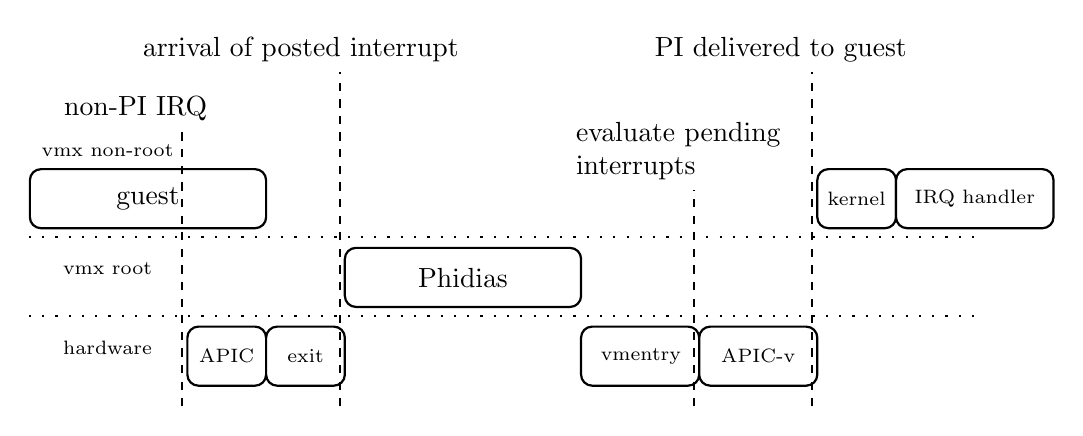
\begin{tikzpicture}

%\draw[step=1cm, gray, very thin, dotted] (0,0) grid (12,4);

\draw[black, thick, loosely dotted] (0,0.9) -- (12,0.9) node at (12,0.9) [below] {};
\draw[black, thick, loosely dotted] (0,1.9) -- (12,1.9) node at (12,1.9) [below] {};
\node at (1, 3) {\scriptsize{vmx non-root}};
\node at (1, 1.5) {\scriptsize{vmx root}};
\node at (1, 0.5) {\scriptsize{hardware}};


\node at (0,2) [rectangle, draw=black, thick, fill=white, rounded corners, minimum height = 0.75cm, minimum width = 3cm, anchor=south west] (gbefore) {guest};
\node at (2,0) [rectangle, draw=black, thick, fill=white, rounded corners, minimum height = 0.75cm, minimum width = 1cm, anchor=south west] (apic) {\scriptsize{APIC}};
\node at (3,0) [rectangle, draw=black, thick, fill=white, rounded corners, minimum height = 0.75cm, minimum width = 1cm, anchor=south west] (vmexit) {\scriptsize{exit}};
\node at (4,1) [rectangle, draw=black, thick, fill=white, rounded corners, minimum height = 0.75cm, minimum width = 3cm, anchor=south west] (phidias1) {Phidias};
\node at (7,0) [rectangle, draw=black, thick, fill=white, rounded corners, minimum height = 0.75cm, minimum width = 1.5cm, anchor=south west, text width=1cm] (entry) {\scriptsize{vmentry}};
\node at (8.5,0) [rectangle, draw=black, thick, fill=white, rounded corners, minimum height = 0.75cm, minimum width = 1.5cm, anchor=south west] (apicv) {\scriptsize{APIC-v}};

\draw[black, thick, dashed] (1.95,-0.25) -- (1.95, 3.25)  node [above, text width = 3cm] {non-PI IRQ};
\draw[black, thick, dashed] (3.95,-0.25) -- (3.95, 4.0)  node [above, text width = 5cm] {arrival of posted interrupt};
\draw[black, thick, dashed] (8.45,-0.25) -- (8.45, 2.5)  node [above, text width = 3cm] {evaluate pending interrupts};
\draw[black, thick, dashed] (9.95,-0.25) -- (9.95, 4.0)  node [above, text width = 4cm] {PI delivered to guest};

\node at (10,2) [rectangle, draw=black, thick, fill=white, rounded corners, minimum height = 0.75cm, minimum width = 1cm, anchor=south west] (gafter) {\scriptsize{kernel}};
\node at (11,2) [rectangle, draw=black, thick, fill=white, rounded corners, minimum height = 0.75cm, minimum width = 2cm, anchor=south west] (irqhandler) {\scriptsize{IRQ handler}};

\end{tikzpicture}
\end{center}
\caption{Posted interrupt worst case scenario}
\label{fig-pii-worstcase}
\end{figure}



\section{Portioning Last Level Cache}
Intel Cache Allocation Technology enables portioning of LLC (L3 cache).
The details of this feature has already been covered in section \ref{sec:cat}.
In short a set of registers called bitmasks allow hypervisor to configure isolated or shared cache regions.
A bit in the bitmask register can correspond to a way in set-associative cache.
A separate register is used to assign portion of the cache to an application based on an identifier called class of service (CLOS).
The Xeon E5-2600v4 processor used to conduct experiments has 15MB 20-way set associative cache bitmask registers has length of 20bits. 
It supports up to 15 CLOS identifiers.
Succeeding sections describe the methodology and records results of using cache allocation technique.


\subsection{Methodology}
The latency reduction is evaluated by measuring worst-case interrupt latency with and without LLC partitioning between the two guests.
The setup includes PREEMPT\_RT patched Linux as real-time guest (rt-guest)
and Linux as general-purpose guest (gp-guest). 
Each guest is assigned to a separate core and has access to 256MB of RAM.
The setup is similar to the one described in section \ref{sec:methodology}, rt-guest has direct access to PCIe gpio card capable to generate interrupts. 
Measurement setup is same as described in section \ref{sec:measurement-setup}.
Phidias hypervisor is extended to support portioning of L3 cache. 
The cache was divided equally between the two guests.
The gpio interrupt latency was measured while high memory demands were generate by gp-guest. 
The experiments were repeated with and without cache allocation to measure improvement in latency.
A synthetic application was used to generate high memory demands from gp-guest.

\subsection{Latency Reduction}
\begin{figure}[!htb]
\begin{center}
\begin{tikzpicture}  [
						my brace/.style={thick, decorate, decoration={brace, amplitude=2pt, raise=10pt,},},							
						my label/.style={below right, align=center, rotate=90, inner ysep=14pt, },
					]

		\begin{axis} [ name=plot1, height=\figheight, width=\figwidth, 
				   enlarge y limits={upper,value=0.3},  enlarge x limits=0.12,
				   ymin=0,
		           %axis y line*=left,
				   ybar=\ybarSep,  
				   x=\ybarXdist,
				   bar width=\ybarWidth,
	   			   ylabel={worst-case interrupt latency ($\mu{}s$)},
	 		       symbolic x coords={no load, cache\_pressure, forkops, fileops, threadops},
		           xtick=data,                 
		            %nodes near coords, 
					%nodes near coords align={vertical}, 
					x tick label style={rotate=0, anchor=north}, 
					xticklabel style={rotate=0,anchor=north, font=\ttfamily\small},
		            xtick align=inside,
		            xticklabel pos=left,
	   			    legend pos=north east, legend columns=-1,
				] 
		\addplot [fill=yellow!20, postaction={pattern=north east lines}, pattern color=gray] coordinates {
				(no load, 67.6)				
				(cache\_pressure, 73.7)
				(forkops, 25.9)
				(fileops, 24.7)
				(threadops, 12.4)
		      };                  

		\addplot [fill=NavyBlue!50, xshift=\xShiftLatency] coordinates {
                     (no load,141.3) 
					(cache\_pressure,132)	
					(forkops,129.9)
					(fileops,123.7)
					(threadops,146.1)
			      }
					coordinate [pos=0] (a1)
		            coordinate [pos=0.2] (a2)
		            coordinate [pos=0.4] (a3)
		            coordinate [pos=0.8] (a4)
		            coordinate [pos=1] (a5)
				  ;

		\addplot [fill=ForestGreen!60, xshift=\xShiftLatency, postaction={pattern=crosshatch dots}, pattern color=gray] coordinates {
                    (no load,120.4) 
					(cache\_pressure,112.2)	
					(forkops,108.4)
					(fileops,106.8)
					(threadops,116.9)
			      }				  	
					coordinate [pos=0] (b1)
		            coordinate [pos=0.2] (b2)
		            coordinate [pos=0.4] (b3)
		            coordinate [pos=0.8] (b4)
		            coordinate [pos=1] (b5)	
				  ;

				  \draw [my brace] (a1) -- (b1) node [my label] {\small{$+14.8\%$}};
				  \draw [my brace] (a2) -- (b2) node [my label] {\small{$+8.8\%$}};
				  \draw [my brace] (a3) -- (b3) node [my label] {\small{$+16.6\%$}};
				  \draw [my brace] (a4) -- (b4) node [my label] {\small{$+13.7\%$}};
				  \draw [my brace] (a5) -- (b5) node [my label] {\small{$+20.0\%$}};
		\legend{native, LLC shared, LLC partitioned}
		\end{axis}

		%%improvement%% 
		%% \begin{axis} [ name=plot1, height=\figheight, width=\figwidth, ybar,  enlarge y limits={upper,value=0.3},  enlarge x limits=0.12, 					
		%% 		   ymin=0, ymax=80,
		%%            axis y line*=right,
		%% 		   ybar=\ybarSep,  
		%% 		   x=\ybarXdist,
		%% 		   bar width=\ybarWidth,
	   	%% 		   ylabel={improvement \%},
	 	%% 	       symbolic x coords={no load, cache pressure, forkops, fileops, threadops},
		%%            xtick=data,                 
		%%             nodes near coords, 
		%% 			nodes near coords align={vertical}, 
		%% 			x tick label style={rotate=0, anchor=north}, 
		%% 			xticklabel style={rotate=0,anchor=north},
		%%             xtick align=inside,
		%%             xticklabel pos=left,
	   	%% 		    legend pos=north east, legend columns=-1,
		%%          ]  
		%% \addplot [fill=OliveGreen!50, xshift=\xShiftImprove, postaction={pattern=crosshatch dots}] coordinates {
        %%             (no load, 14.8) 
		%% 			(cache pressure,8.8)	
		%% 			(forkops,16.6)
		%% 			(fileops,13.7)
		%% 			(threadops,20)
		%% 	      };
		%% \legend{improvement}
		%% \end{axis}

%%%%%%%%%%%%%%%%%%for defense presentation%%%%%%%%%%%%%%%%%%%%
\ifdefense

\end{tikzpicture}
\end{center}
\label{plot-cat1}
\end{figure}
	
\begin{figure}[!htb]
\begin{center}
\begin{tikzpicture}  [
						my brace/.style={thick, decorate, decoration={brace, amplitude=2pt, raise=10pt,},},							
						my label/.style={below right, align=center, rotate=90, inner ysep=14pt, },
					]

\fi
%%%%%%%%%%%%%%%%%%%%%ENDIF%%%%%%%%%%%%%%%%%%%%%%%%%%%%%%%%%
	\begin{axis} [ name=plot2, \atCmdLowerPlot, 
					height=\figheight, width=\figwidth, enlarge y limits={upper,value=0.3},  
					enlarge x limits=0.12,
				   ymin=0,
		           %axis y line*=left,
				   ybar=\ybarSep,
				   x=\ybarXdist,
				   bar width=\ybarWidth,
	   			   ylabel={average-case interrupt latency ($\mu{}s$)},
	 		       symbolic x coords={no load, cache\_pressure, forkops, fileops, threadops},
		           xtick=data,                 
		            %nodes near coords, 
					%nodes near coords align={vertical}, 
					x tick label style={rotate=0, anchor=north, font=\ttfamily\small}, 
					xticklabel style={rotate=0,anchor=north},
		            xtick align=inside,
		            xticklabel pos=left,
	   			    legend pos=north east, legend columns=-1,
				 ] 
		\addplot [fill=yellow!20, postaction={pattern=north east lines}, pattern color=gray] coordinates {
				(no load, 44.2)				
				(cache\_pressure, 43.1)
				(forkops, 6.1)
				(fileops, 6.1)
				(threadops, 5)
			   };  
                   
		\addplot [fill=NavyBlue!50, xshift=\xShiftLatency] coordinates {
                    (no load,19.1) 
					(cache\_pressure,28.5)	
					(forkops,13.1)
					(fileops,13.8)
					(threadops,19.6)			
			      }
					coordinate [pos=0] (a1)
		            coordinate [pos=0.2] (a2)
		            coordinate [pos=0.4] (a3)
		            coordinate [pos=0.8] (a4)
		            coordinate [pos=1] (a5)
				  ;
		\addplot [fill=ForestGreen!60, xshift=\xShiftLatency, postaction={pattern=crosshatch dots}, pattern color=gray] coordinates {
                     (no load,15.7) 
					(cache\_pressure,15.2)	
					(forkops,9.9)
					(fileops,10)
					(threadops,12.4)			
			      }				  	
					coordinate [pos=0] (b1)
		            coordinate [pos=0.2] (b2)
		            coordinate [pos=0.4] (b3)
		            coordinate [pos=0.8] (b4)
		            coordinate [pos=1] (b5)	
				  ;

				  \draw [my brace] (a1) -- (b1) node [my label] {\small{$+17.8\%$}};
				  \draw [my brace] (a2) -- (b2) node [my label] {\small{$+46.6\%$}};
				  \draw [my brace] (a3) -- (b3) node [my label] {\small{$+24.4\%$}};
				  \draw [my brace] (a4) -- (b4) node [my label] {\small{$+27.5\%$}};
				  \draw [my brace] (a5) -- (b5) node [my label] {\small{$+36.7\%$}};
	\legend{native, LLC shared, LLC partitioned}
	\end{axis}

	%%improvement%%
	%% \begin{axis} [ name=plot2, \atCmdLowerPlot,  height=\figheight, width=\figwidth, ybar,  
	%% 				enlarge y limits={upper,value=0.3},  enlarge x limits=0.12, ymin=0, ymax=80,
	%% 	           axis y line*=right,
	%% 			   ybar=\ybarSep,  
	%% 			   x=\ybarXdist,             
	%% 			   bar width=\ybarWidth,
	%%    			   ylabel={improvement \%},
	%%  		       symbolic x coords={no load, cache pressure, forkops, fileops, threadops},
	%% 	           xtick=data,                 
	%% 	            nodes near coords, 
	%% 				nodes near coords align={vertical}, 
	%% 				x tick label style={rotate=0, anchor=north}, 
	%% 				xticklabel style={rotate=0,anchor=north},
	%% 	            xtick align=inside,
	%% 	            xticklabel pos=left,
	%%    			    legend pos=north east, legend columns=-1,
	%% 	         ]  
	%% \addplot [fill=OliveGreen!50, xshift=\xShiftImprove, postaction={pattern=crosshatch dots}] coordinates {
    %%                 (no load,17.8) 
	%% 				(cache pressure,46.6)	
	%% 				(forkops,24.4)
	%% 				(fileops,27.5)
	%% 				(threadops,36.7)
	%% 		      };
	%% \legend{improvement}
	%% \end{axis}

\end{tikzpicture}
\end{center}
\ifreport
\caption{Interrupt latency comparison of shared LLC and partitioned LLC}
\label{plot-cat}
\else
\label{plot-cat2}
\fi
\end{figure}


The latency measurement experiment was repeated for different load conditions on rt-guest when gp-guest was executed application large amounts of memory. 
Figure \ref{plot-cat} plots comparison of worst-case and average-case interrupt latencies when LLC is shared and when it is partitioned. 
It is clear that separating real-time guest cache from the other guest improves both worst-case and average-case interrupt response times.
The best results are observed when guest is loaded with \mforkops{} benchmark. 
Interrupt latency reduced approximately by $21us$ with $16\%$ improvement.

%\section{Isolating TLB Traffic}
\section{TLB Virtualization} \label{sec:vtlb-latency-red}
Translation lookaside buffers (TLBs) are used by the processor to cache virtual to physical address translations.
Modern architectures have  separate TLBs for instruction and data known as iTLB and dTLB respectively. 
In a virtual environment hypervisor and guest operating system access different virtual address spaces.
Caching translations of both address spaces at same TLB can result in thrashing translations of each other on context switch. 
Furthermore when a guest flushes TLB entries, it also flushes cached information for hypervisor address space.
Hypervisor can use TLB virtualization through VPIDs to isolate traffic of its own address space from the guests running in virtual machines.
This section evaluates performance improvement for interrupt response time by using VPIDs.

\subsection{Methodology}
Two guest setup from the previous section is used again, however this time hypervisor is extended to use VPID mechanism.
Hypervisor assigns a unique process identifier to each guest and emulates TLB flush instructions for the guest 
based on VPIDs. The guest is oblivious to VPID mechanism.
Note that performance evaluation is focused on isolating guest translations from hypervisor as both execute on the same core.
Since Phidias hypervisor uses multikernel approach the shared resources are at least used by hypervisor and the guest.

The latency reduction is evaluated by measuring worst-case interrupt latency with and without TLB virtualization.
The setup includes PREEMPT\_RT patched Linux as real-time guest (rt-guest)
and Linux as general-purpose guest (gp-guest). 
The setup is similar to the one described in section \ref{sec:methodology}, rt-guest has direct access to PCIe gpio card capable to generate interrupts. 
Measurement setup is same as described in section \ref{sec:measurement-setup}.
Hypervisor was extended to support TLB virtualization. 
It assigns a unique process identifier to each guest and emulates TLB flush instructions for the guest based on VPIDs.

\subsection{Latency Reduction}

\begin{figure}[!htb]
\begin{center}
\begin{tikzpicture}  [
						my brace/.style={thick, decorate, decoration={brace, amplitude=3pt, raise=4pt,},},							
						my label/.style={below right, align=center, rotate=90, inner ysep=10pt, },
						another label/.style={below right, align=center, rotate=90, inner ysep=5pt, },
					]

	\begin{axis} [ name=plot1, height=\figheight, width=\figwidth, 
				   enlarge y limits={upper,value=0.3},  enlarge x limits=0.12,
				   ymin=0,
		           %axis y line*=left,
				   ybar=\ybarSep,  
				   x=\ybarXdist,
				   bar width=\ybarWidth,
	   			   ylabel={worst-case  latency ($\mu{}s$)},
	 		       symbolic x coords={no load, cache\_pressure, forkops, fileops, threadops},
		           xtick=data,                 
		            %nodes near coords, 
					%nodes near coords align={vertical}, 
					x tick label style={rotate=0, anchor=north, font=\ttfamily\small}, 
					xticklabel style={rotate=0,anchor=north},
		            xtick align=inside,
		            xticklabel pos=left,
	   			    legend pos=north east, legend columns=-1,
				 ]                    
	\addplot [fill=NavyBlue!50, xshift=\xShiftLatency] coordinates {
                    (no load,129.5) 
					(cache\_pressure,145.6)	
					(forkops,128.2)
					(fileops,127.1)
					(threadops,169.6)
			      }
					coordinate [pos=0] (a1)
		            coordinate [pos=0.2] (a2)
		            coordinate [pos=0.4] (a3)
		            coordinate [pos=0.8] (a4)
		            coordinate [pos=1] (a5)
				  ;

	\addplot [fill=ForestGreen!60, xshift=\xShiftLatency, postaction={pattern=crosshatch dots}, pattern color=gray] coordinates {
                    (no load,130.5) 
					(cache\_pressure,131.7)	
					(forkops,124.8)
					(fileops,123.7)
					(threadops,148.8)
			      }
				  	coordinate [pos=0] (b1)
		            coordinate [pos=0.2] (b2)
		            coordinate [pos=0.4] (b3)
		            coordinate [pos=0.8] (b4)
		            coordinate [pos=1] (b5)	
				  ;

				  \draw [thick, |-|] ([xshift=4pt]a1) -- ([xshift=4pt]b1) node [another label] {\small{$-0.8\%$}};
				  \draw [thick, |-|] ([xshift=4pt]a2) -- ([xshift=4pt]b2) node [another label] {\small{$+9.5\%$}};
				  \draw [thick, |-|] ([xshift=4pt]a3) -- ([xshift=4pt]b3) node [another label] {\small{$+2.6\%$}};
				  \draw [thick, |-|] ([xshift=4pt]a4) -- ([xshift=4pt]b4) node [another label] {\small{$+2.7\%$}};
				  \draw [my brace] (a5) -- (b5) node [my label] {\small{$+12.2\%$}};
	\legend{shared TLB, isolated TLB}
	\end{axis}

	%%improvement%%
	%% \begin{axis} [ name=plot1, height=\figheight, width=\figwidth, ybar,  enlarge y limits={upper,value=0.3},  enlarge x limits=0.12, 					
	%% 			   ymin=0, ymax=80,
	%% 	           axis y line*=right,
	%% 			   ybar=\ybarSep,  
	%% 			   x=\ybarXdist,
	%% 			   bar width=\ybarWidth,
	%%    			   ylabel={improvement \%},
	%%  		       symbolic x coords={no load, cache pressure, forkops, fileops, threadops},
	%% 	           xtick=data,                 
	%% 	            nodes near coords, 
	%% 				nodes near coords align={vertical}, 
	%% 				x tick label style={rotate=0, anchor=north}, 
	%% 				xticklabel style={rotate=0,anchor=north},
	%% 	            xtick align=inside,
	%% 	            xticklabel pos=left,
	%%    			    legend pos=north east, legend columns=-1,
	%% 	         ]  
	%% 	\addplot [fill=OliveGreen!50, xshift=\xShiftImprove, postaction={pattern=crosshatch dots}] coordinates {
    %%                 (no load, 0) 
	%% 				(cache pressure,9.5)	
	%% 				(forkops,2.6)
	%% 				(fileops,2.7)
	%% 				(threadops,12.2)
	%% 		      };
	%% 	\legend{improvement}
	%% 	\end{axis}
%%%%%%%%%%%%%%%%%%for defense presentation%%%%%%%%%%%%%%%%%%%%
\ifdefense

\end{tikzpicture}
\end{center}
\label{plot-vpid1}
\end{figure}
	
\begin{figure}[!htb]
\begin{center}
\begin{tikzpicture} [
						my brace/.style={thick, decorate, decoration={brace, amplitude=3pt, raise=4pt,},},							
						my label/.style={below right, align=center, rotate=90, inner ysep=10pt, },
					]

\fi
%%%%%%%%%%%%%%%%%%%%%ENDIF%%%%%%%%%%%%%%%%%%%%%%%%%%%%%%%%%

		\begin{axis} [	 name=plot2, \atCmdLowerPlot, 
					height=\figheight, width=\figwidth, enlarge y limits={upper,value=0.3},  
					enlarge x limits=0.12,
				   ymin=10,
		           %axis y line*=left,
				   ybar=\ybarSep,
				   x=\ybarXdist,
				   bar width=\ybarWidth,
	   			   ylabel={average-case latency ($\mu{}s$)},
	 		       symbolic x coords={no load, cache\_pressure, forkops, fileops, threadops},
		           xtick=data,                 
		            %nodes near coords, 
					%nodes near coords align={vertical}, 
					x tick label style={rotate=0, anchor=north}, 
					xticklabel style={rotate=0,anchor=north, font=\ttfamily\small},
		            xtick align=inside,
		            xticklabel pos=left,
	   			    legend pos=north east, legend columns=-1,
					]                    
		\addplot [fill=NavyBlue!50, xshift=\xShiftLatency] coordinates {
                    (no load,18.2) 
					(cache\_pressure,18.1)	
					(forkops,12.6)
					(fileops,14.5)
					(threadops,17)			
			      }
					coordinate [pos=0] (a1)
		            coordinate [pos=0.2] (a2)
		            coordinate [pos=0.4] (a3)
		            coordinate [pos=0.8] (a4)
		            coordinate [pos=1] (a5)
				  ;
		\addplot [fill=ForestGreen!60, xshift=\xShiftLatency, postaction={pattern=crosshatch dots}, pattern color=gray] coordinates {
                    (no load,17) 
					(cache\_pressure,16.7)	
					(forkops,11.6)
					(fileops,13.4)
					(threadops,15.4)			
			      }
				  	coordinate [pos=0] (b1)
		            coordinate [pos=0.2] (b2)
		            coordinate [pos=0.4] (b3)
		            coordinate [pos=0.8] (b4)
		            coordinate [pos=1] (b5)	
				  ;

				  \draw [my brace] (a1) -- (b1) node [my label] {\small{$+6.5\%$}};
				  \draw [my brace] (a2) -- (b2) node [my label] {\small{$+7.7\%$}};
				  \draw [my brace] (a3) -- (b3) node [my label] {\small{$+7.9\%$}};
				  \draw [my brace] (a4) -- (b4) node [my label] {\small{$+7.5\%$}};
				  \draw [my brace] (a5) -- (b5) node [my label] {\small{$+9.4\%$}};
		\legend{shared TLB, isolated TLB}
		\end{axis}

	%%improvement%%
	%% \begin{axis} [ name=plot2, \atCmdLowerPlot,  height=\figheight, width=\figwidth, ybar,  
	%% 				enlarge y limits={upper,value=0.3},  enlarge x limits=0.12, ymin=0, ymax=80,
	%% 	           axis y line*=right,
	%% 			   ybar=\ybarSep,  
	%% 			   x=\ybarXdist,             
	%% 			   bar width=\ybarWidth,
	%%    			   ylabel={improvement \%},
	%%  		       symbolic x coords={no load, cache pressure, forkops, fileops, threadops},
	%% 	           xtick=data,                 
	%% 	            nodes near coords, 
	%% 				nodes near coords align={vertical}, 
	%% 				x tick label style={rotate=0, anchor=north}, 
	%% 				xticklabel style={rotate=0,anchor=north},
	%% 	            xtick align=inside,
	%% 	            xticklabel pos=left,
	%%    			    legend pos=north east, legend columns=-1,
	%% 	         ]  
	%% \addplot [fill=OliveGreen!50, xshift=\xShiftImprove, postaction={pattern=crosshatch dots}] coordinates {
    %%                 (no load,6.5)
	%% 				(cache pressure,7.7)	
	%% 				(forkops,7.9)
	%% 				(fileops,7.5)
	%% 				(threadops,9.4)
	%% 		      };
	%% \legend{improvement}
	%% \end{axis}

\end{tikzpicture}
\end{center}
\ifreport
\caption{Interrupt latency comparison of shared and isolated TLB between guest and Phidias}
\label{plot-vpid}
\else
\label{plot-vpid2}
\fi
\end{figure}



The latency measurement experiment was repeated for different load conditions on real-time guest and no load on gp-guest. 
Figure \ref{plot-vpid} plots comparison of worst-case and average-case interrupt latencies with shared and isolated TLBs for rt-guest and hypervisor. 
Results show that separating guest TLB using VPID mechanism has improved both the worst-case and average-case interrupt latencies.
The average-case interrupt latency has decreased by at least $1.1us$. The worst-case latency has slightly increased with no load condition,
however it has always decreased with load conditions. 
The best results are produced when guest is loaded with \mthreadops{} benchmark. 
Interrupt latency reduced by approximately $20us$ with $12\%$ improvement.

\section{Putting it Altogether}
This section records improvement in real-time interrupt latency when all latency reduction techniques are combined.
Figure \ref{plot-allopt} plots comparison of average and worst-case interrupt latencies between virtualization overhead recorded in later 
chapter and latency reduction techniques presented in this chapter.
\begin{figure}[!htb]
\begin{center}
\begin{tikzpicture} %[scale = 1.2]

\begin{axis} [name=plot1, height=7cm, width=14cm, ybar=2pt, enlarge y limits={upper,value=0.3},  %enlargelimits=0.3, 
			ymin=0,
			legend pos=north east, legend columns=-1,
                       %legend style={at={(0.5,-0.1)}, anchor=north, legend columns=-1}, 
                       ylabel={worst-case latency(us)}, %title=no pollution from gp-guest, 
		       bar width= 24pt,
			%symbolic x coords={without VPID, with VPID},
                       symbolic x coords={no load, cache pressure, forkops, fileops, threadops},
                       xtick=data, nodes near coords, nodes near coords align={vertical}, x tick label style={rotate=0,anchor=north}, ]                    
	\addplot [fill=black!50] coordinates {
                    (no load,130.8) 
					(cache pressure,141.7)	
					(forkops,119.5)
					(fileops,146.4)
					(threadops,169.1)
			      };

	\addplot [postaction={pattern=north east lines}] coordinates {
                    (no load,97.7) 
					(cache pressure,102.2)	
					(forkops,93.6)
					(fileops,100.7)
					(threadops,96.8)
			      };
\legend{without optimization, latency reduction techniques}
\end{axis}


\begin{axis} [name=plot2, at={($(plot1.west)+(0,-9cm)$)}, height=7cm,  width=14cm, ybar=2pt, enlarge y limits={upper,value=0.3},  %enlargelimits=0.3, 
			ymin=0,
                       legend pos=north east, legend columns=-1,
			%legend style={at={(0.5,-0.1)}, anchor=north, legend columns=-1}, 
                       ylabel={average-case latency (us)}, %title=no pollution from gp-guest, 
		       bar width= 24pt,
                       %symbolic x coords={without VPID, with VPID},
			symbolic x coords={no load, cache pressure, forkops, fileops, threadops},
                       xtick=data, nodes near coords, nodes near coords align={vertical}, x tick label style={rotate=0,anchor=north}, ]                    
	\addplot [fill=black!50] coordinates {
                    (no load,18.2) 
					(cache pressure,26.6)	
					(forkops,12.6)
					(fileops,14.3)
					(threadops,16.4)			
			      };
	\addplot [postaction={pattern=north east lines}] 				
				coordinates {
                    (no load,11) 
					(cache pressure,10.9)	
					(forkops,7.6)
					(fileops,7.7)
					(threadops,9.6)			
			      };
\legend{without optimization, latency reduction techniques}
\end{axis}

\end{tikzpicture}

%\begin{tabular}{c c c c c}
%\multicolumn{5}{c}{Percentage Improvement}
%no load & cache pressure & forkops & fileops & threadops \\
%25.3 & 27.9 & 21.7 & 31.2 & 42.8 \\
%\end{tabular}

\end{center}
\ifreport
\caption{Comparison of interrupt latency when no optimization is deployed versus latency reduction techniques (direct interrupt, cache allocation, isolated TLB cache)}
\fi
\label{plot-allopt}
\end{figure}



The interrupt response time has improved approximately $30\%$ when latency reduction techniques are deployed.
The overall improvement with all optimization enabled look very similar to results for direct interrupt mechanism, however there is slight improvement in average-case and worst-case.

Figure \ref{plot-cdf-native-virtual-optimiz} plots CDF of gpio interrupt latency for three different setups: native, virtual with no optimization and virtual with latency reduction techniques. The interrupt latency is plotted for three different loads, same as in Figure \ref{plot-cdf-native-vs-virtual}.
The comparison of CDFs reveals improved average-case response time and reduced spread compared with virtualization overhead recorded in previous chapter.

\begin{figure}[!htb]
\begin{center}

\begin{tikzpicture}


\begin{axis}[name=plot1, height=6cm, width=12cm, ymin=0, ymax=1, xmin=0, 		
		xlabel=latency(us), 
		ylabel=probability,
		title style={yshift=-2ex},
		legend pos=south east,
		title=load:cache pressure,
		]
	\addplot [thick, blue] table[x=Latency,y=Probability] {./figures/native_cachepressure_10k_cdf.dat};
	\addplot [thick, red] table[x=Latency,y=Probability] {./figures/virt_cachepressure_10k_cdf.dat};
	\addplot [very thick, green] table[x=Latency,y=Probability] {./figures/allopt_cachepressure_10k_cdf.dat};
	\legend {\small{native (avg 44.2, max 77.9)}, \small{virtual (avg 18.2, max 131.1)}, \small{optimized (avg 11, max 100.4)}}
\end{axis}


\begin{axis}[name=plot2, at={($(plot1.south west)+(0,-6.5cm)$)}, height=6cm, width=12cm, ymin=0, ymax=1, xmin=0, 
		legend pos=south east,
		xlabel=latency(us), 
		ylabel=probability, 
		title style={yshift=-2ex},
		title=load:threadops,
		]
	\addplot [thick, blue] table[x=Latency,y=Probability] {./figures/native_threadops_cdf.dat};	
	\addplot [thick, red] table[x=Latency,y=Probability] {./figures/virt_threadops_10k_cdf.dat};
	\addplot [very thick, green] table[x=Latency,y=Probability] {./figures/allopt_threadops_10k_cdf.dat};
	\legend {\small{native (avg 5, max 12.4)}, \small{virtual (avg 16.4, max 169.1)}, \small{optimized (avg 9.6, max 96.8)}}
\end{axis}



\begin{axis}[name=plot3, at={($(plot2.south west)+(0,-6.5cm)$)}, height=6cm, width=12cm, ymin=0, ymax=1, xmin=0, 
		legend pos=south east,
		xlabel=latency(us), 
		ylabel=probability, 
		title style={yshift=-2ex},
		title=load:forkops,
		]
	\addplot [thick, blue] table[x=Latency,y=Probability] {./figures/native_forkops_10k_cdf.dat};	
	\addplot [thick, red] table[x=Latency,y=Probability] {./figures/virt_forkops2_10k_cdf.dat};
	\addplot [very thick, green] table[x=Latency,y=Probability] {./figures/allopt_forkops_10k_cdf.dat};
	\legend {\small{native (avg 6.1, max 25.9)}, \small{virtual (avg 12.6, max 119.5)}, \small{optimized (avg 7.6, max 97.7)}}
\end{axis}

\end{tikzpicture}
\end{center}
\ifreport
\caption{Comparison of interrupt latency CDF between native and virtual setup for different load conditions}
\fi
\label{plot-cdf-native-virtual-optimiz}
\end{figure}





